\documentclass[10pt, aspectratio=169, compress]{beamer}
\usetheme[progressbar=frame title, numbering=fraction]{metropolis}      % Use metropolis theme 
\setbeamertemplate{section in toc}[sections numbered]
\setbeamertemplate{subsection in toc}[subsections numbered]
\useoutertheme[subsection=false]{miniframes}
\setbeamercolor{section in head/foot}{fg=white, bg=mDarkTeal}
\setbeamercolor{background canvas}{bg=white}
\setbeamerfont{section in head/foot}{series=\bfseries}

\usefonttheme[onlymath]{serif}
\usepackage{amsmath}
\usepackage{remreset}
\usepackage{ragged2e}
\usepackage{booktabs}
\usepackage{makecell}
\usepackage{float}
\usepackage{subfig}
\usepackage{tikz}
\usetikzlibrary{positioning,calc,trees}
\usepackage[flushleft]{threeparttable}	% 3 part table 
\usepackage[justification=centering]{caption}
\captionsetup{skip=0pt}
\graphicspath{{./fig/}}

\makeatletter
\let\beamer@writeslidentry@miniframeson=\beamer@writeslidentry
\def\beamer@writeslidentry@miniframesoff{%
	\expandafter\beamer@ifempty\expandafter{\beamer@framestartpage}{}% does not happen normally
	{%else
		% removed \addtocontents commands
		\clearpage\beamer@notesactions%
	}
}
\newcommand*{\miniframeson}{\let\beamer@writeslidentry=\beamer@writeslidentry@miniframeson}
\newcommand*{\miniframesoff}{\let\beamer@writeslidentry=\beamer@writeslidentry@miniframesoff}
\beamer@compresstrue
\makeatother

%==============================================================
% Title Page
%==============================================================
%Information to be included in the title page:
\title{Análisis de Datos}
\subtitle{Construcción de Datos}
\author{Rony Rodriguez-Ramírez} 
\institute{LAMBDA}
\titlegraphic{\hfill
\includegraphics[height=1.5cm]{dime}}
\date{\today}
%==============================================================
\begin{document}
%------------------------------------------------	
\begin{frame}[plain]
	\maketitle 
\end{frame}
%------------------------------------------------
\section{Introducción}
%-----------------------------------------------
\subsection{Introducción}
%-----------------------------------------------
\begin{frame}[t]{Inputs}
	\textbf{Constructed dataset:}
	\begin{itemize}
		\item Incluir solo las variables necesarias para el análisis
		\item Libro de códigos de acompañamiento con descripción y definición de variables.
		\item Hecho a medida para responder sus preguntas de análisis
		\begin{itemize}
			\item Muestra
			\item Unidad de observación
		\end{itemize}
	\end{itemize}
\end{frame}
%-----------------------------------------------
\begin{frame}[t]{Outputs}
	\begin{itemize}
		\item Los resultados son exportados a archivos que pueden ser vistos como inputs para papers o reportes.
		\item Tablas independientes y gráficos. 
		\item Formatos accesibles.
	\end{itemize}
\end{frame}
%-----------------------------------------------
\begin{frame}[t]{Outputs}
	\begin{itemize}
		\item Los resultados finales, como documentos, informes breves e incluso creados para analizar los resultados, deben actualizarse automáticamente cuando se actualizan los resultados sin procesar.
		\item \LaTeX es una herramienta extremadamente útil para hacer esto.
		\item Si no sabe cómo usarlo, consulte nuestra capacitación en \LaTeX de DIME.
	\end{itemize}
\end{frame}
%-----------------------------------------------
\begin{frame}{Documentación}
	\begin{itemize}
		\item Otro resultado importante del análisis es un mapa de cómo se crearon los resultados
		\item El script maestro (master do file) es la mejor manera de hacer esto: debe hacer un seguimiento de lo que son las entradas y salidas de cada script que ejecuta.
		\item Un archivo README también es una buena forma de hacerlo, especialmente cuando se usan idiomas de programación y software específicos.
	\end{itemize}
\end{frame}
%-----------------------------------------------
\section{Análisis}
%-----------------------------------------------
\subsection{Análisis}
%-----------------------------------------------
\begin{frame}{El proceso de Análisis}
	\begin{itemize}[<+->]
		\item El análisis de datos se puede dividir en dos etapas.
		\item Durante el análisis \textbf{exploratorio de datos}, el equipo de investigación generalmente buscará patrones en los datos, de manera más descriptiva.
		\item El proceso luego avanza hacia el \textbf{análisis final} cuando el equipo comienza a decidir cuáles son los resultados principales, que formarán parte del resultado de la investigación.
		\item Para los proyectos que tienen planes de preanálisis, las especificaciones principales se predefinirán, por lo que la fase exploratoria tiene menos implicaciones para los resultados finales.
	\end{itemize}
\end{frame}
%-----------------------------------------------
\begin{frame}{Trabajo de datos durante el análisis}
	\begin{itemize}[<+->]
		\item La forma en que maneja el código y los resultados para el análisis exploratorio y final es diferente.
		\item Durante el análisis exploratorio de datos, estará tentado a escribir muchos análisis en un gran script, o incluso directamente en la consola.
		\item Esto fomenta sutilmente prácticas riesgosas como no limpiar el espacio de trabajo y no recargar los datos relevantes.
		\item Para evitar errores, es importante tomarse el tiempo para organizar el código que desea usar de nuevo de manera limpia.
	\end{itemize}
\end{frame}
%-----------------------------------------------
\begin{frame}
	\frametitle{Documentos dinámicos durante el análisis exploratorio}
	\begin{itemize}
		\item Una forma de evitar caer en malas prácticas durante el análisis exploratorio de datos es crear documentos dinámicos
		\item Le permiten escribir código, tomar notas sobre sus observaciones y visualizar resultados en un solo documento
		\item Las opciones de Stata incluyen \texttt{markstat}, que usa una sintaxis similar a markdown, y \texttt{texdoc}, que combina código \LaTeX y Stata
		\item En R, \texttt{RMarkdown} es ampliamente adoptado
		\item La principal limitación de este tipo de documentos dinámicos son las opciones de formato limitadas que se ofrecen y la dificultad de manejar código y texto al mismo tiempo.
	\end{itemize}
\end{frame}
%-----------------------------------------------
\begin{frame}
	\frametitle{Documentos dinámicos durante el análisis final}
	\begin{itemize}
		\item Dadas las limitaciones de crear documentos dinámicos en software estadístico, el equipo tiende a preferir pasar al editor de texto o a los sistemas de preparación de documentos para escribir los resultados finales de la investigación.
		\item Al configurar este flujo de trabajo, es importante pensar en la integración entre las salidas de código y el texto.
	\end{itemize}
\end{frame}
%-----------------------------------------------
\begin{frame}
	\frametitle{Documentos dinámicos durante el análisis final}
	\begin{itemize}
		\item El código generalmente sigue evolucionando a medida que se redactan los documentos e informes, y es importante mantener los resultados del código actualizados en los documentos finales
		\item \LaTeX es la forma más popular de hacer esto
		\item Le permite escribir referencias a los archivos que contienen resultados de análisis, para que se actualicen cada vez que se compila el documento \LaTeX.
	\end{itemize}
\end{frame}	
%-----------------------------------------------
\section{Un workflow automatizado}
%-----------------------------------------------
\subsection{Un workflow automatizado}
%-----------------------------------------------
\begin{frame}
	\frametitle{Exportando outputs}
	\begin{itemize}
		\item Está bien no exportar todas y cada una de las tablas y gráficos creados durante el análisis exploratorio.
		\item Los resultados finales deben exportarse para que estén listos para ser incluidos en un documento o informe.
		\item No deberían ser necesarias ediciones manuales, incluido el formateo, después de exportar los resultados finales.
		\item No cree un flujo de trabajo que implique copiar y pegar en diferentes programas.
	\end{itemize}
\end{frame}
%-----------------------------------------------
\begin{frame}
	\frametitle{Automatizando outputs}
	\begin{itemize}
		\item Las ediciones manuales son difíciles de replicar e inevitablemente necesitará realizar cambios en los resultados.
		\item La cantidad de trabajo necesaria en un flujo de trabajo de copiar y pegar aumenta rápidamente con el número de resultados, y también lo hacen las posibilidades de que la versión incorrecta resulte en su documento o informe.
		\item Automatizar la creación de resultados le ahorrará tiempo al final del proceso.
		\item Los resultados finales de pulido pueden llevar mucho tiempo
		\item No pase demasiado tiempo formateando hasta que su equipo haya acordado los resultados finales.
	\end{itemize}
\end{frame}
%-----------------------------------------------
\begin{frame}
	\frametitle{En caso que no sea claro...}
	
	\begin{center}
		{\LARGE 
		Nunca configure un flujo de trabajo que requiera copiar y pegar resultados.
		}
	\end{center}
\end{frame}
%-----------------------------------------------
\begin{frame}
	\frametitle{Automatizando outputs}
	\begin{itemize}[<+->]
		\item Copiar resultados de Excel a Word es propenso a errores e ineficiente.
		\item La copia de los resultados de una consola de software es aún más ineficiente y es completamente innecesaria.
		\item Existen numerosos comandos para exportar salidas de R y Stata a una miríada de formatos.
		\item Nuestro comando Stata preferido para exportar tablas son \texttt{esttab}, \texttt{outreg2} y \texttt{outwrite}.
		\item Nuestro paquete R preferido para exportar tablas es \texttt{stargazer}.
		\item ¡Hay muchos más por ahí!
	\end{itemize}	
\end{frame}
%-----------------------------------------------
\begin{frame}
	\frametitle{Automatizando outputs}
	\begin{itemize}
		\item \texttt{estout} puede resovler la mayoría de los problemas. 
		\item Puede exportar tanto summary statistics y tablas de regresión de una manera sencilla. 
		\item También suportar bastante tipos de customización, y exporta tanto a Excel como a \LaTeX.
	\end{itemize}
\end{frame}
%-----------------------------------------------
\begin{frame}
	\frametitle{Automatizando outputs}
	
	Puede encontrar más ejemplo en los siguientes repositorios: 
	\begin{enumerate}
		\item \href{https://github.com/bbdaniels/stata-tables}{https://github.com/bbdaniels/stata-tables}
		\item \href{https://github.com/RRMaximiliano/stata-latex-tables}{https://github.com/RRMaximiliano/stata-latex-tables}
	\end{enumerate}
\end{frame}
%-----------------------------------------------
\begin{frame}
	\frametitle{Automatizando outputs}
	\begin{itemize}
		\item También puede editar el conjunto de datos directamente y exportar los datos a Excel con exportación de Excel, a csv con exportación delimitada o a \LaTeX con salida de datos
		\item Si te apetece, puedes crear matrices y exportarlas usando \texttt{mat2txt} o sobrescribir.
		\item Finalmente, puede exportar \texttt{tabulaciones} de una y dos vías usando \texttt{tabout}.
	\end{itemize}	
\end{frame}
%-----------------------------------------------
\section{Escribiendo scripts de análisis}
\subsection{Escribiendo scripts de análisis}
%-----------------------------------------------
\begin{frame}
	\frametitle{Organización del script (do file)}
	Un scripts (do file) muy bien ordenado:
	\begin{itemize}[<+->]
		\item Comienza con un espacio de trabajo completamente nuevo.
		\item Carga el conjunto de datos construido.
		\item Toma decisiones de investigación explícitamente (muestreo, agrupamiento, inclusión de controles).
		\item Tiene un código simple que permite al usuario enfocarse en la econometría.
		\item Exporta los resultados obtenidos.
		\item Se ejecuta de forma completamente independiente de todos los demás códigos, excepto el script maestro.
		\item Se puede vincular a su salida por nombre.
	\end{itemize}
\end{frame}
%-----------------------------------------------
\begin{frame}
	\frametitle{Organización del script (do file)}
	\begin{itemize}[<+->]
		\item El código de análisis debe ser limpio y simple: incluso puede crear un script para cada salida
		\item Si tiene múltiples conjuntos de datos de análisis, cada uno de ellos debe tener un nombre descriptivo sobre su muestra y unidad de observación, por lo que está claro qué conjunto de datos se debe utilizar para cada análisis.
		\item En ambos casos, la denominación debe ser intuitiva para que pueda rastrear las entradas y salidas de cada script.
	\end{itemize}
\end{frame}
%-----------------------------------------------
\begin{frame}
	\frametitle{Organización del script (do file)}
	\begin{itemize}[<+->]
		\item Cuando su equipo toma decisiones sobre la especificación del modelo, puede crear globales u objetos en la secuencia de comandos maestra para usar en las secuencias de comandos.
		\item Esto asegurará que las especificaciones sean consistentes durante todo el análisis.
		\item También hará que su código sea más dinámico, por lo que es fácil actualizar las especificaciones y los resultados sin cambiar cada script.
		\item Utilice comandos preexistentes siempre que sea posible: evite abarrotar su código con comandos complicados para crear y agregar matrices intermedias.
	\end{itemize}
\end{frame}
%-----------------------------------------------
\section{Outputs finales}
\subsection{Outputs finales}
%-----------------------------------------------
\begin{frame}
	\frametitle{¡Mira tu outputs!}
	\begin{itemize}
		\item ¿El aspecto es decente?
		\item ¿Alguien más puede entenderlo?
		\item Verifique el número de observaciones
		\item Pregúntese si los resultados tienen sentido
		\item Verifique nuevamente el número de observaciones
		\item Intenta interpretar el resultado
		\item Verifique las escalas
	\end{itemize}
\end{frame}
%-----------------------------------------------
\begin{frame}
	\frametitle{¡Mira tu outputs!}

	\begin{center}
		{
		\LARGE
			Al escribir un artículo pregúntese: ¿sus tablas y figuras despiertan alegría?
		}
	\end{center}
\end{frame}
%-----------------------------------------------
\begin{frame}
	\frametitle{¿Ahora qué?}

	\begin{itemize}[<+->]
		\item Si sigue los pasos descritos en este capítulo, la mayoría del trabajo de datos involucrado en el último paso del proceso de investigación - publicación - ya estará hecho.
		\item Su código de análisis se organizará de manera reproducible, por lo que todo lo que necesitará para lanzar un paquete de replicación es una última ronda de revisión de código.
		\item Esto te permitirá concentrarte en lo que importa: escribir tus resultados en una historia convincente
	\end{itemize}
\end{frame}

%==============================================================
% Stata TIME
%==============================================================
\miniframesoff 	

\begin{frame}[plain, noframenumbering]
	\begin{center}
	\LARGE STATA TIME
		\begin{figure}[H]
			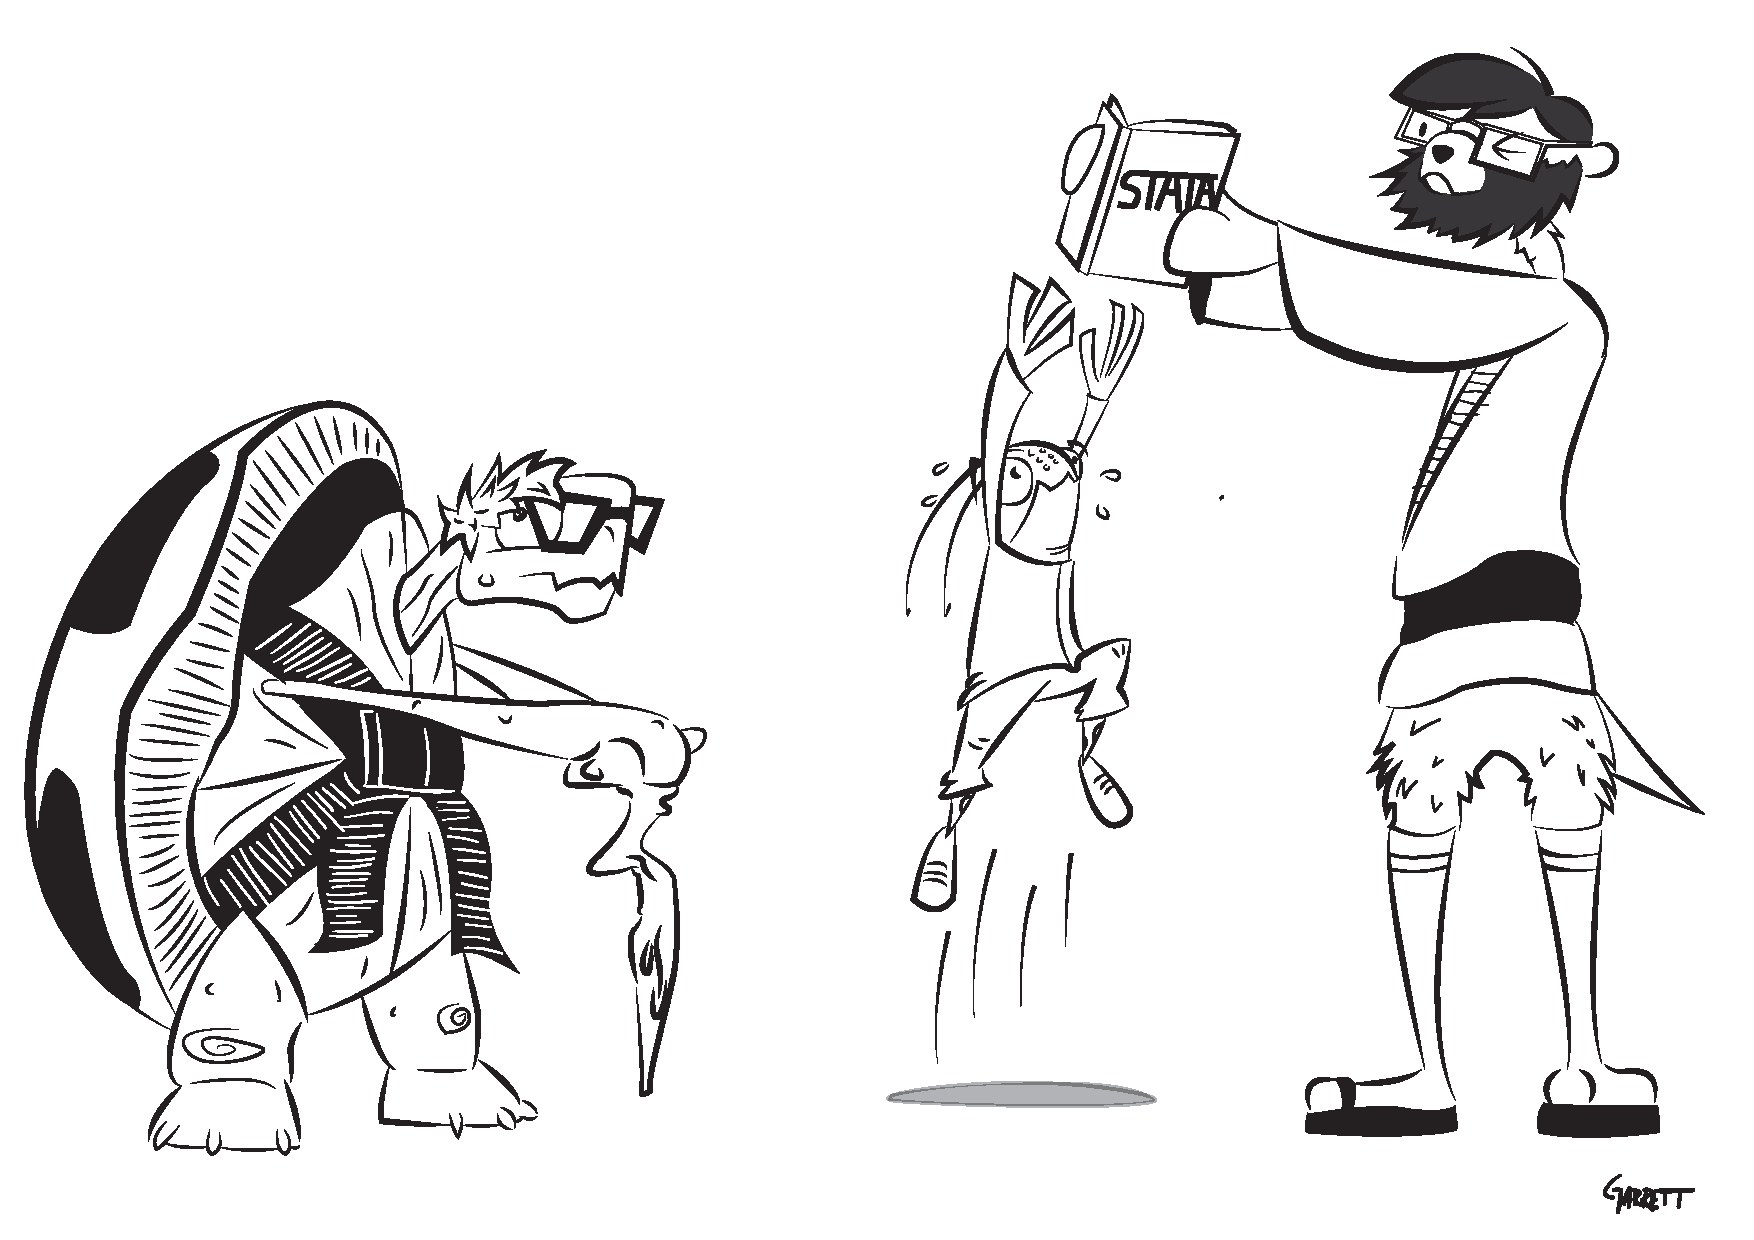
\includegraphics[width=0.57\textwidth]{stata.pdf}
		\end{figure}
	\end{center}
\end{frame}
%==============================================================
% END
%==============================================================	
\begin{frame}[plain, standout]
	Nos vemos mañana.
\end{frame}
%-----------------------------------------------
\end{document}		
